\documentclass[12pt]{article}

% Specify document formatting.
\renewcommand{\baselinestretch}{1.5} 
\usepackage[top=2.5cm,bottom=2.5cm,inner=4cm,outer=2.5cm,twoside]{geometry}
\usepackage{fancyhdr} \usepackage{pdfpages} \usepackage[nottoc,notlof,notlot,numbib]{tocbibind}

% Change section title font size to 14.
\usepackage{sectsty}
\sectionfont{\fontsize{14}{15}\selectfont}

\usepackage{fontspec}
\setmainfont{Times New Roman}

\usepackage{amsmath} \usepackage{graphicx} \usepackage{microtype} \usepackage{float}
\usepackage[hidelinks]{hyperref} \usepackage{cleveref}
\usepackage{siunitx} \usepackage{gensymb}
\usepackage{tabularx} \usepackage{booktabs}
\usepackage[style=ieee]{biblatex} \addbibresource{zotero.bib}

\begin{document}
\includepdf{title.pdf}
\thispagestyle{empty}
\pagebreak

\pagenumbering{roman}
\section*{Abstract}
%\addcontentsline{toc}{section}{Abstract}
\pagebreak

\renewcommand{\contentsname}{Table of Contents}
\tableofcontents
\listoffigures
\listoftables
\pagebreak

\pagenumbering{arabic}
\section{Introduction}
% Powered wheelchairs do this.
% Smart wheelchairs do this.
% Indoor vs Outdoor assistance.
% Sensors
% Machine Learning
%\cite{tomariEnhancingWheelchairControl2014}
\pagebreak

\section{Aims}
The aim of this research is to develop a semi-autonomous smart wheelchair system.
This research is done in collaboration with Glide, a WA wheelchair manufacturer,
who have provided an existing powered wheelchair (CentroGlide) to use as a base
for this functionality. By developing assistive technology for the wheelchair,
the user is granted greater mobility, confidence, and independence.

There are multiple engineering research project students who are part of this team,
working on elements such as controller design, navigation assistance, and object detection.
This work specifically focuses on pathway assistance, which identifies suitable
paths for the wheelchair to drive on. If a user unintentionally drives off their desired path,
this can lead to uneven terrain and possibly falling from the wheelchair.
By guiding the user along a path, these safety issues can be mitigated.

Emphasis is placed on the 'semi-autonomous' aspect of the wheelchair.
An important requirement of this project is that the user still
has control over their wheelchair, and can override any semi-autonomous functionality
if required. When false positives occur within the smart wheelchair system,
the users mobility should not be compromised.

Another requirement of the system is that any sensors mounted to the wheelchair
should not impede the users comfort or the wheelchairs manouverability.
Many wheelchair users have specific requirements for wheelchair seat adjustments,
to avoid pressure sores and discomfort. \Cref{fig:wheelchair_reclined} shows the
wheelchair configuration when fully reclined, demonstrating that some sensor mounting locations
are infeasible.

The smart wheelchair system should also be commercially viable. This means that high-cost
components such as 3D LIDAR are infeasible. Internet connectivity should not be a requirement
for the system to operate either - the round trip time required to communicate with a server
would compromise the safety of a user. Because of this, all processing is performed locally
on the wheelchair.

\begin{figure}
    \centering
    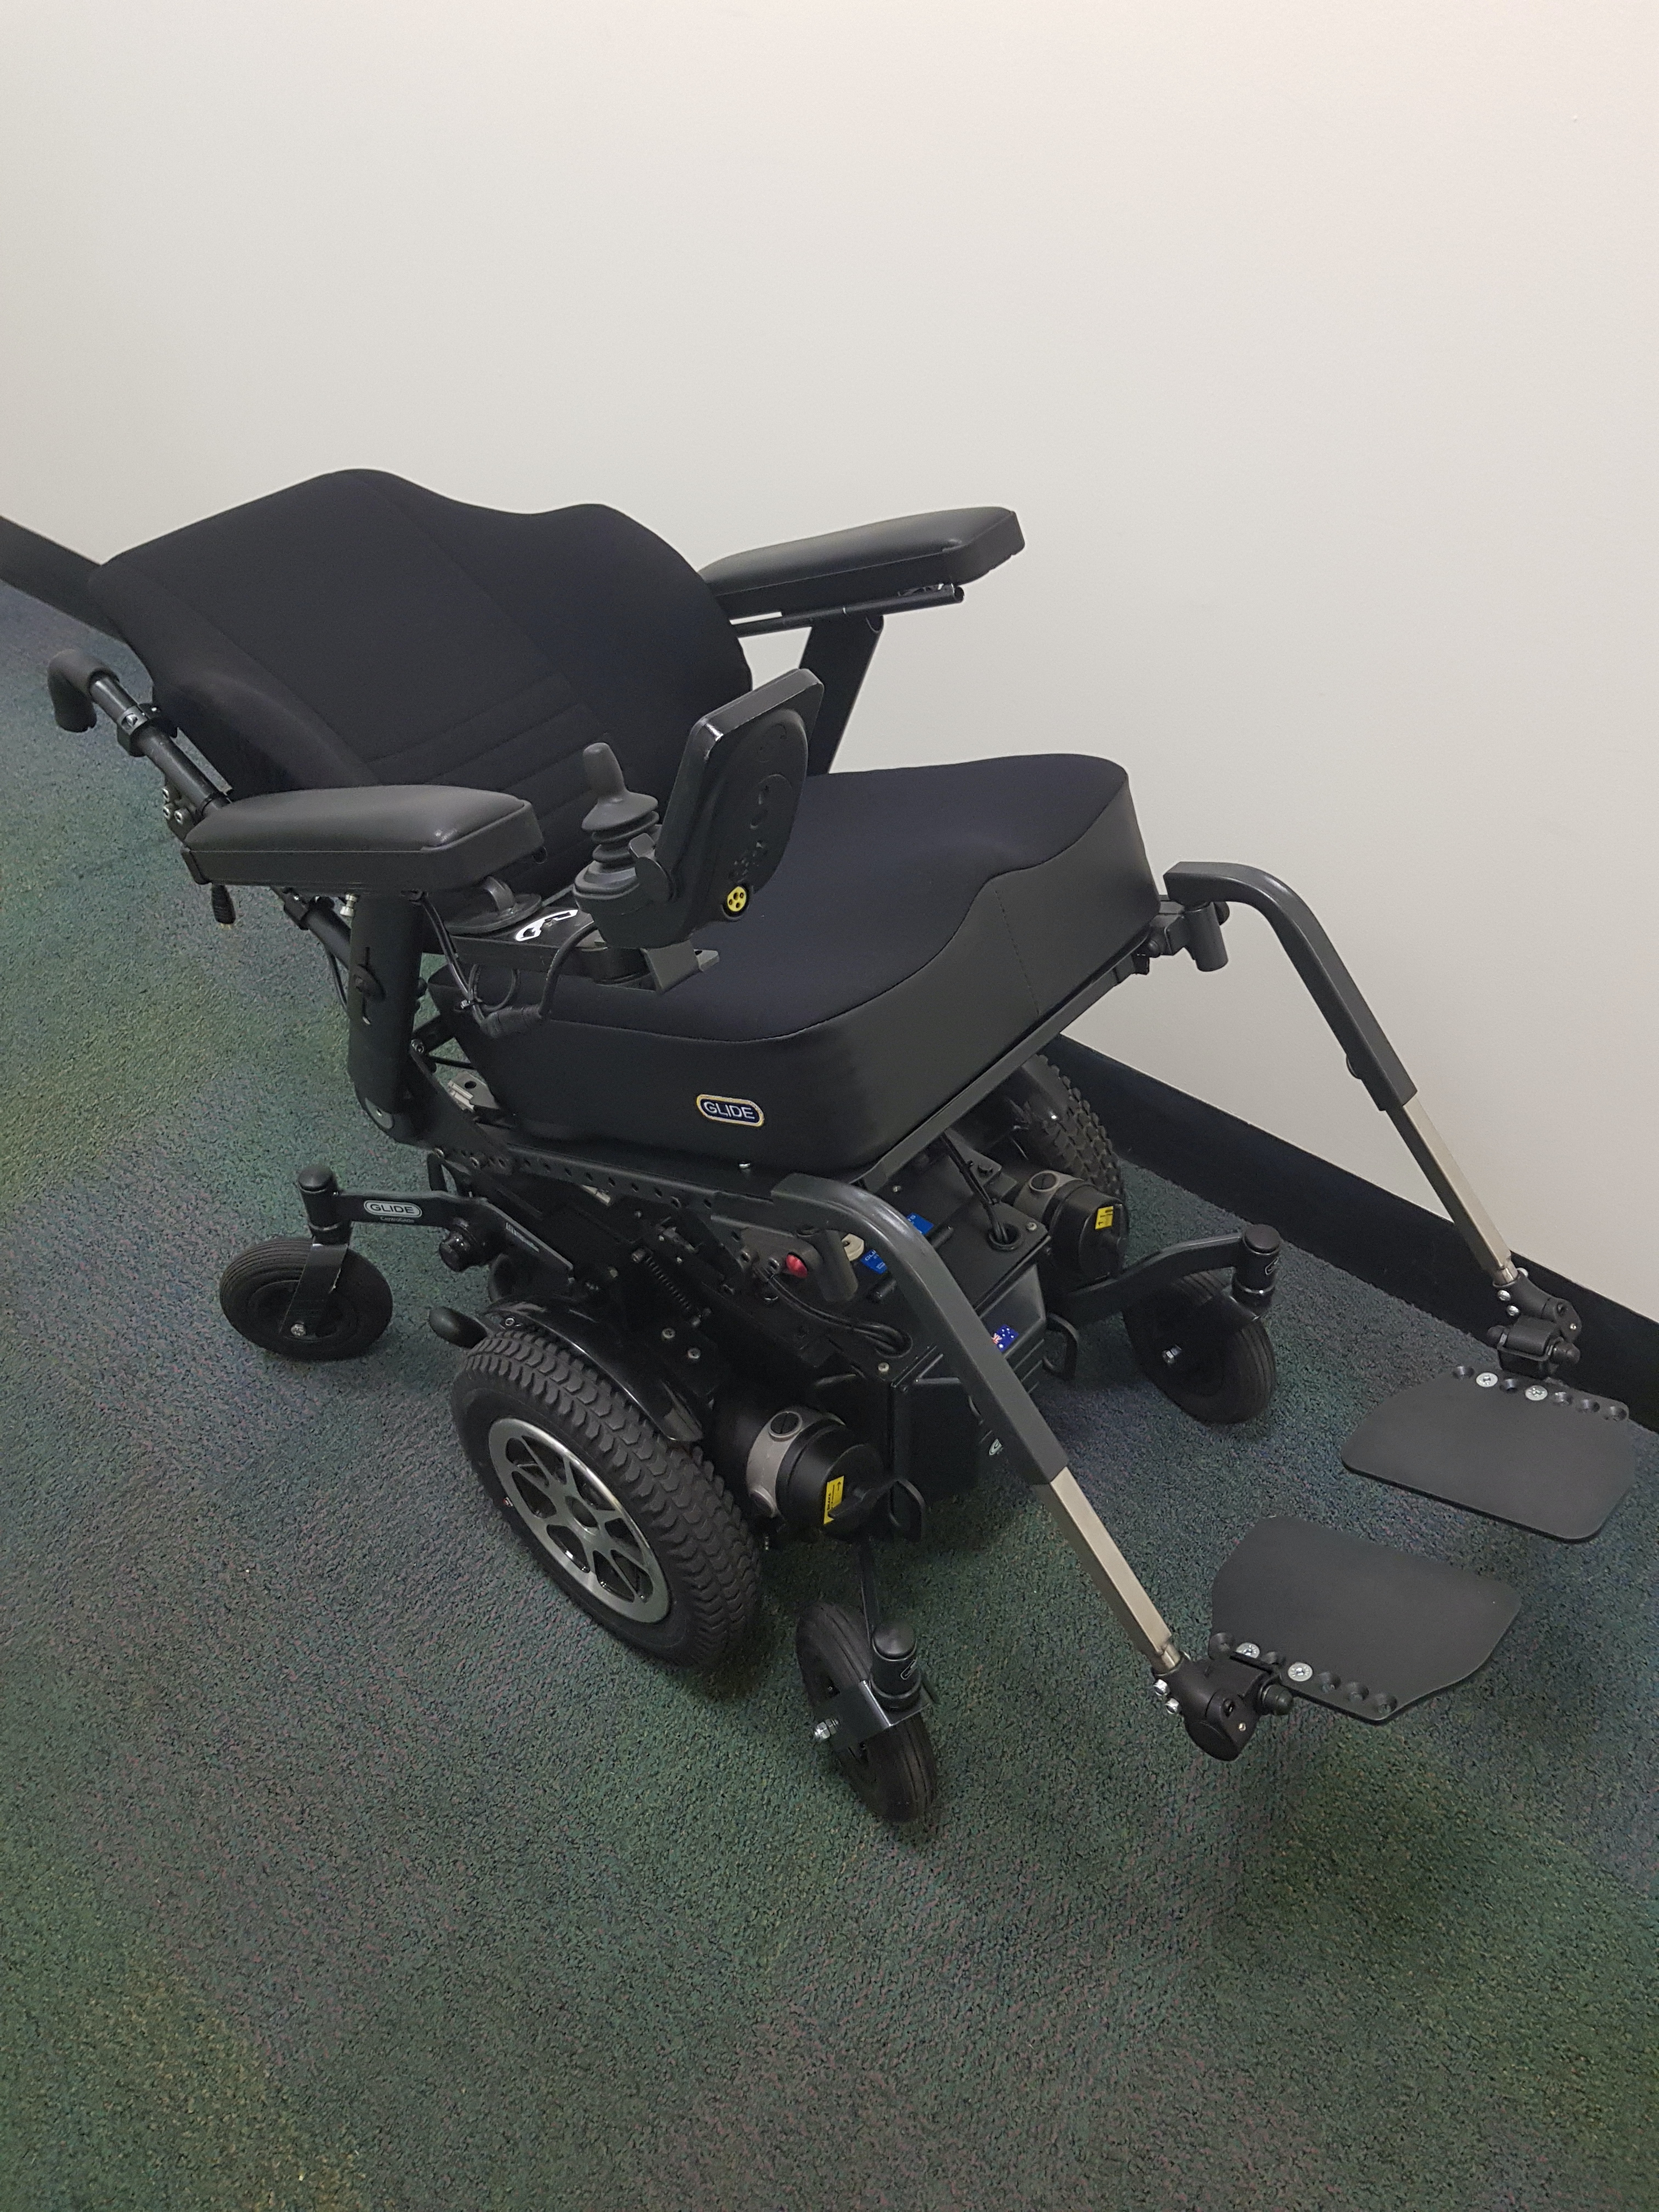
\includegraphics[width=0.8\linewidth]{images/wheelchair_reclined.jpeg}
    \caption{CentroGlide in Reclined Configuration}
    \label{fig:wheelchair_reclined}
\end{figure}

\pagebreak

\section{Results and Discussion}
% 34 minute dataset
The first stages of smart wheelchair development involved:
\begin{enumerate}
    \item Identifying desired sensors and hardware for the wheelchair.
    \item Choosing an appropriate mounting point for these sensors.
    \item Researching the field of machine perception and computer vision (both applied to wheelchairs and more generally).
    \item Collecting an initial video dataset, enabling work to begin on labelling and algorithm evaluation.
\end{enumerate}

\subsection{Hardware}
The smart wheelchair should have the ability to sense, process, and manouver within the surrounding environment.
To do this requires some necessary hardware, including a sensor system, compute element, and motor controller.
Due to the 2021-2022 chip shortage, hardware selection was identified as a process that should occur relatively quickly.

\Cref{table:sensor_options} shows some sensors that were considered for use in the smart wheelchair.
Selecting a sensor to use is not necessarily an either-or decision. Sensor fusion algorithms such as
the Extended Kalman Filter (EKF) or Unscented Kalman Filter (UKF) \cite{wanUnscentedKalmanFilter2000} allow
outputs from multiple sensors to be used together to improve their accuracy. Additionally, some sensors may
be used for different applications on the smart wheelchair.

\begin{table}
    \centering
    \begin{tabular}{c c c}
    \toprule
    Sensor & Advantages & Disadvantages \\
    \midrule
    Stereo Camera & High Resolution & \\
    MMWave Radar & & \\
    3D Lidar & & High Cost \\
    2D Lidar & & \\
    Ultrasonic Radar & & \\
    Inertial Measurement Unit (IMU) & & \\
    Servo Motor Encoder & & \\
    \bottomrule
    \end{tabular}
    \caption{Sensor Comparisons}
    \label{table:sensor_options}
\end{table}

After consideration of the available options, it was decided to use a stereo camera as the main
forward facing sensor, with 2D LIDAR used for the side and rear of the wheelchair.

The front of the joystick control unit was selected as the best mounting point for the
stereo camera, due to several reasons:
\begin{enumerate}
    \item Clear view of the environment in front of the wheelchair.
    \item Not obstructed by the user in any wheelchair configuration.
    \item When needed, the user can move the joystick control unit out of the way,
            which also moves the camera out of the way.
\end{enumerate}

\pagebreak

\section{Future Work}
\pagebreak

\printbibliography[heading=bibnumbered]

\end{document}
